\section{Engagement analysis \label{sec:engagement}}

\import{content/06-evaluation/structured_analysis}{textual_responses.tex}

\subsection{Numeric responses}

In many features, we can further observe the polarizing effects of the competitive design: while in \ac{pv} the responses tend to be more grouped around the center, \ac{cv} have more spread out distributions with more extreme values.

\FloatBarrier
\begin{figure}[ht]
\centering
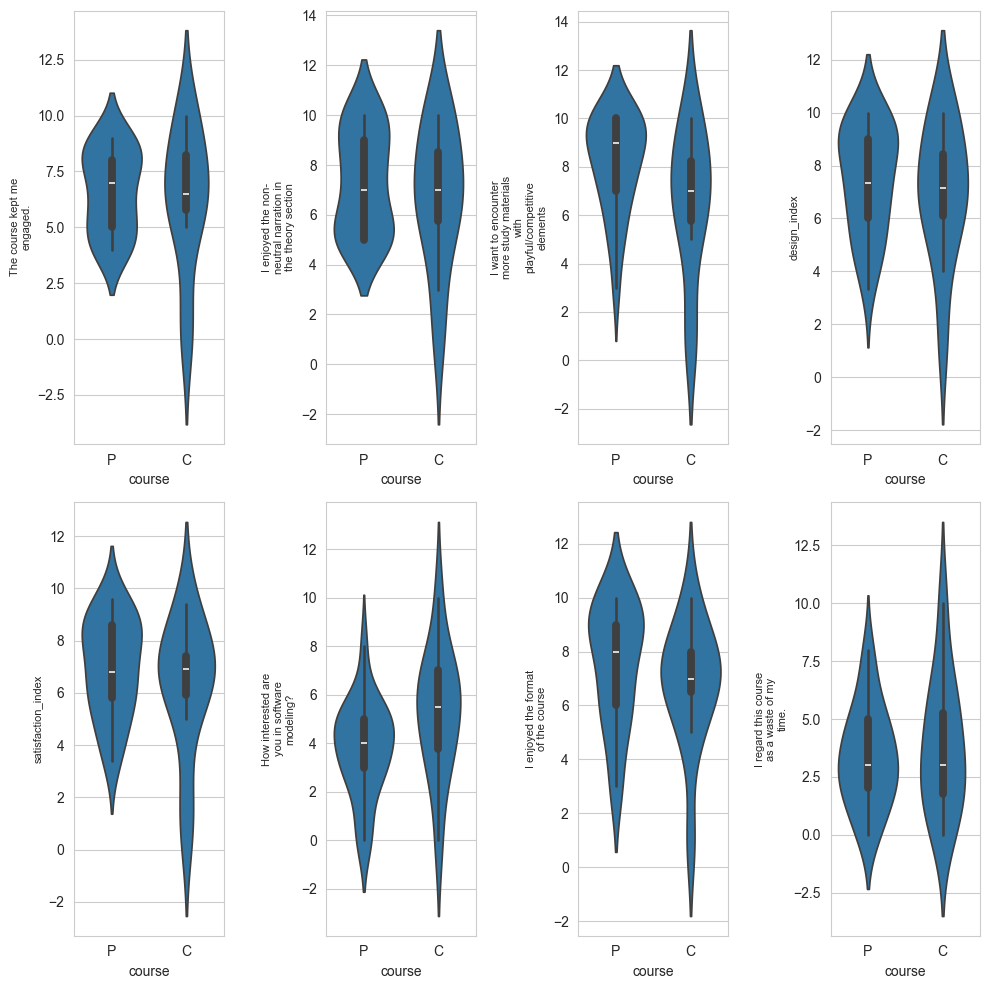
\includegraphics[width=1\textwidth]{assets/images/eval/engagement/engagement_violinplots.png}
\caption{Distributions of subjective metrics in the feedback questionnaire}
\label{fig:engagement_violinplots}
\end{figure}
\FloatBarrier

In most features, \ac{pv} displays higher engagement and satisfaction values than \ac{cv}. That corresponds with observations from open-ended questions in the feedback questionnaire (see Section~\ref{sec:text_feedback}).

\FloatBarrier
\begin{figure}[ht]
\centering
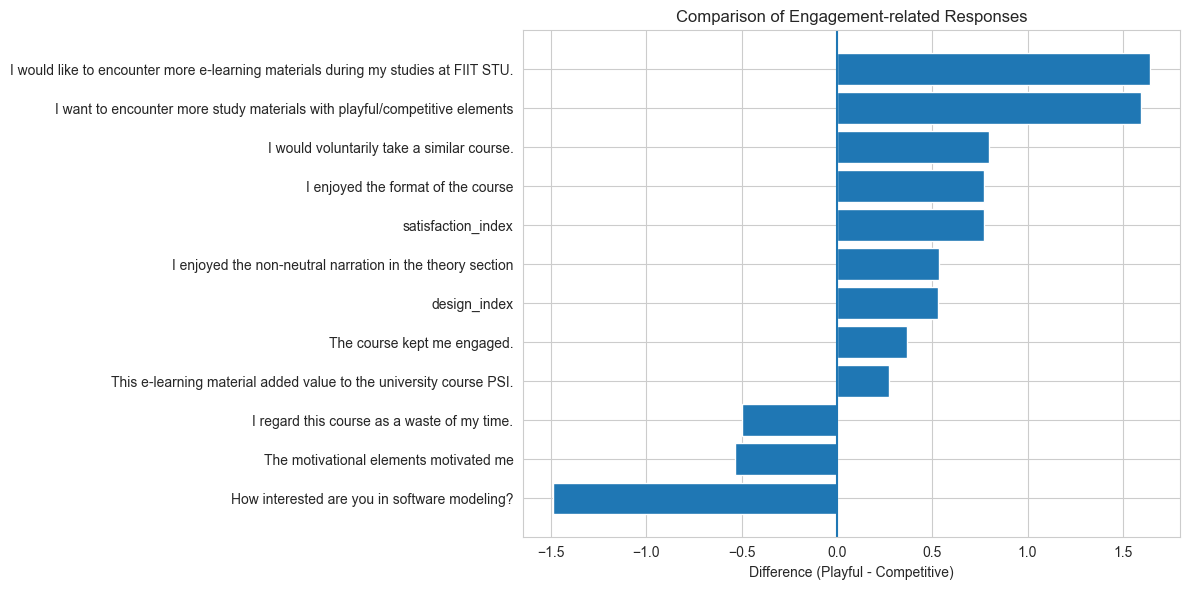
\includegraphics[width=1\textwidth]{assets/images/eval/engagement/engagement_means_comparison.png}
\caption{Difference of means (\ac{pv}-\ac{cv}) in engagement and general satisfaction metrics in the feedback questionnaire}
\label{fig:engagement_means_comparison}
\end{figure}
\FloatBarrier

Despite the higher engagement rates and general satisfaction of participants in \ac{pv}, there is one interesting drawback of the course - while in \ac{cv} the interest in software modeling remained the same before and after the course was taken, \ac{pv} shows a decrease in interest. 
% As the difference is not statistically significant (Mann–Whitney U, p=0.420229,Cohen’s d=-0.316), it might be attributed to coincidence
There are several possible explanations for the observation. Students take the topic less seriously when presented in a playful tone, extrinsic rewards may shift motivation away from intrinsic interest. However, the difference is not statistically significant (Mann–Whitney U, p=0.420229,Cohen’s d=-0.316) and should not be interpreted as a robust effect.

Preference for both competitive and playful elements dropped slightly between the start and end of the courses. The decrease is not statistically significant in either variant (Mann–Whitney U, \ac{pv} - p=0.295627, \ac{cv} - p=0.315938) and can be attributed to discrepancy between what the students imagined as playful or competitive and the content of the courses, and to mental fatigue from the tasks. 

Notably, the difference between the drops roughly corresponds to the difference in answers to the question \enquote{The course kept me engaged} in the feedback questionnaire (see Figure~\ref{fig:engagement_means_comparison}), suggesting a potential relationship between engagement and the drop in preference.

The answer to the questions \enquote{What is your attitude towards competitive activities?} and \enquote{What is your attitude towards playful study materials?} are not in the feedback questionnaire directly - the design\_index value was used instead (see Section~\ref{sec:data_prep}).

\FloatBarrier
\begin{figure}[ht]
\centering
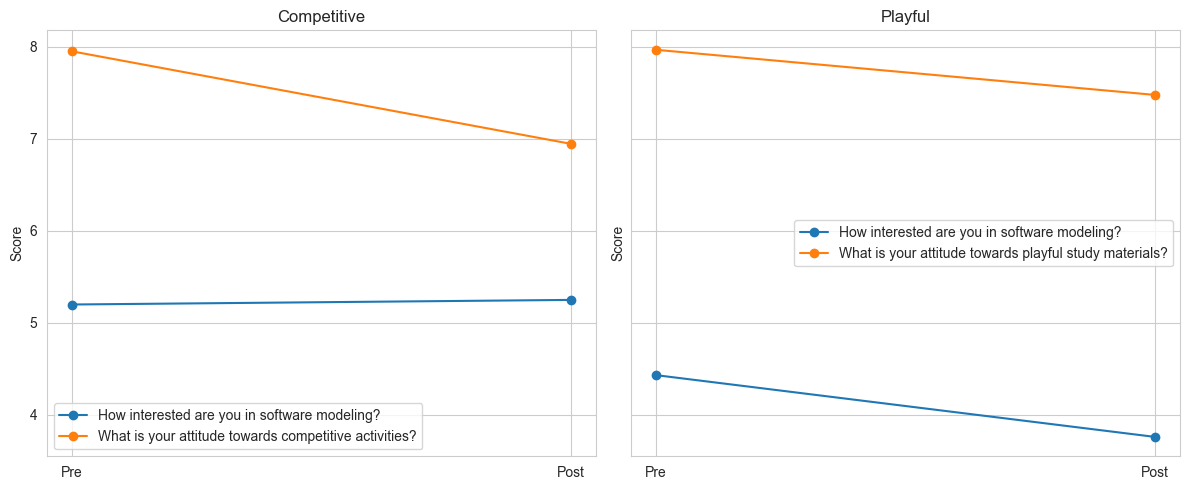
\includegraphics[width=1\textwidth]{assets/images/eval/engagement/interest_pre_post.png}
\caption{Perceptions of student before and after taking the courses}
\label{fig:interest_pre_post}
\end{figure}
\FloatBarrier


In the following correlation matrices we can observe and interesting pattern. In \ac{pv}, there is weak correlation between interest in software modeling and perceived skill level (r=0.17). Interest in playful study materials is largely independent of the other metrics as well.

In contrast, \ac{cv} group shows a strong relationship between interest in software modeling and self-reported \ac{uml} skill (r=0.83). What is noticeable is that enthusiasm for competitive activities is more strongly related (r=0.72) to interest in software modeling rather than perceived skill (r=0.47). This indicates a more tightly coupled response structure, where students who report higher interest in software modeling also tend to report higher perceived competence and more positive attitudes toward competition.

% A possible interpretation of these relationships is that competitive design suits students when they are both interested in the topic and perceive themselves as competent. 

% Assuming the students were responding with the context of software modeling in mind, a potential interpretation is that students enjoy competing in activities if they are interested in them. However, the question is general and more research is needed before making conclusions. The relationship might be random.\todo{are you sure bro this is a weird thing to say}

This coupled with \ac{cv} having lower participation rate and higher baseline skill level suggests that students were more likely to be put off by \ac{cv} - unless already interested and competent. \ac{pv} did not present a barrier for beginner or disinterested students.

% It should be noted, however, that the questionnaire items are phrased in a general manner, which may introduce ambiguity in interpretation and limit the strength of conclusions drawn from these relationships.

\FloatBarrier
\begin{figure}[ht]
\centering
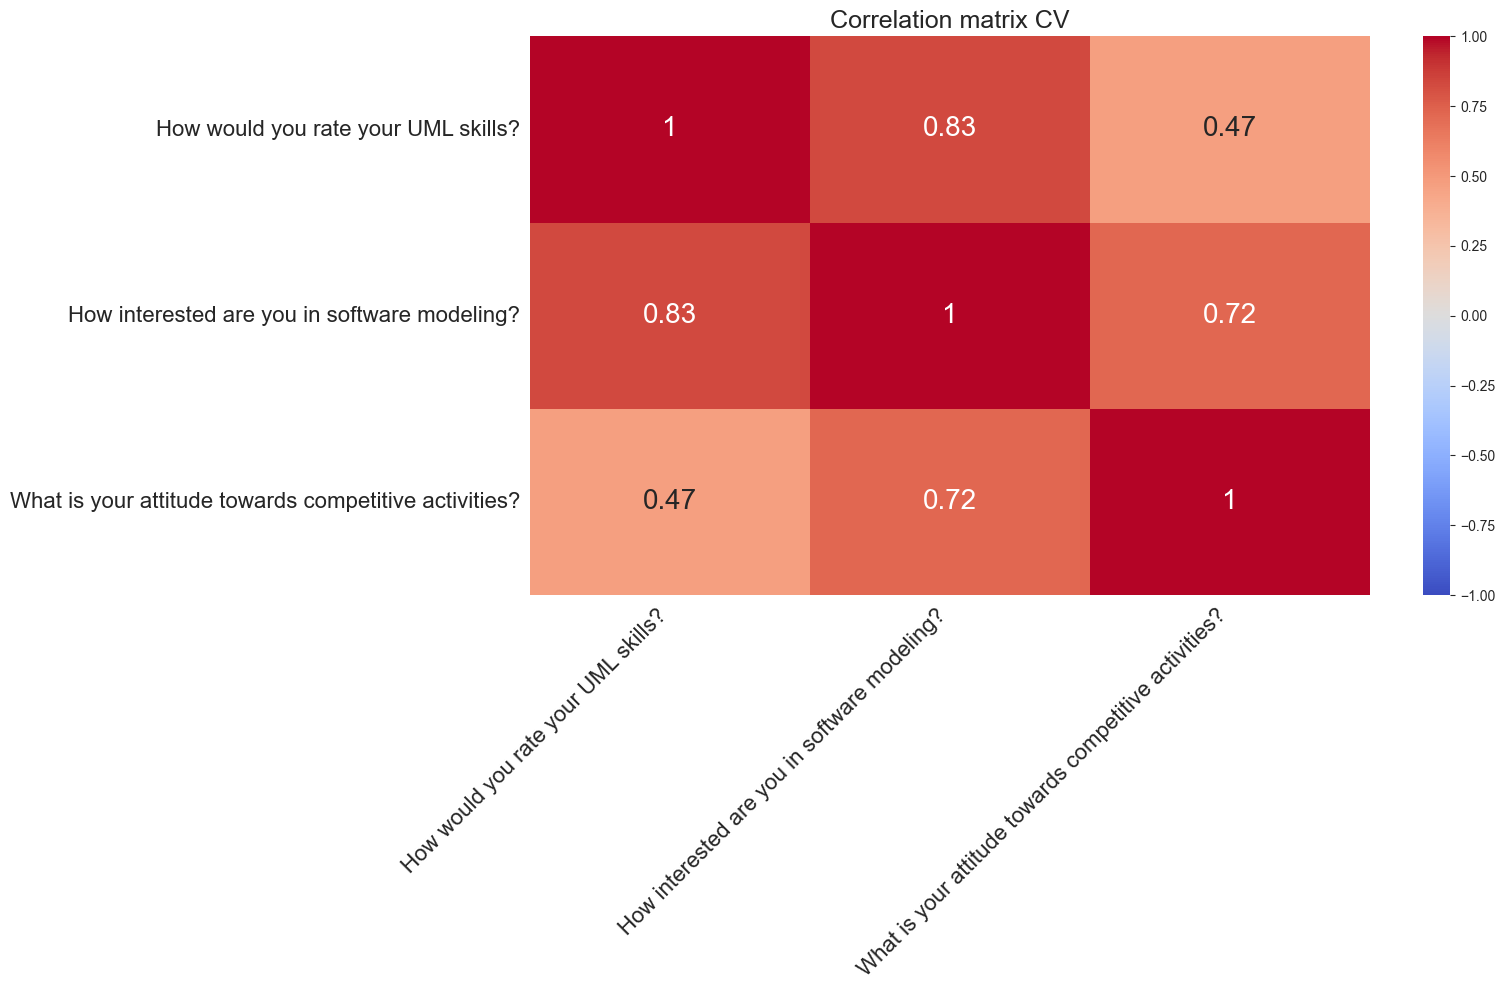
\includegraphics[width=0.85\textwidth]{assets/images/eval/engagement/corr_matrix_feedback_C_1.png}
\caption{Correlation matrix for feedback questionnaire - \ac{cv}}
\label{fig:corr_matrix_feedback_C_1}
\end{figure}
\FloatBarrier

\FloatBarrier
\begin{figure}[ht]
\centering
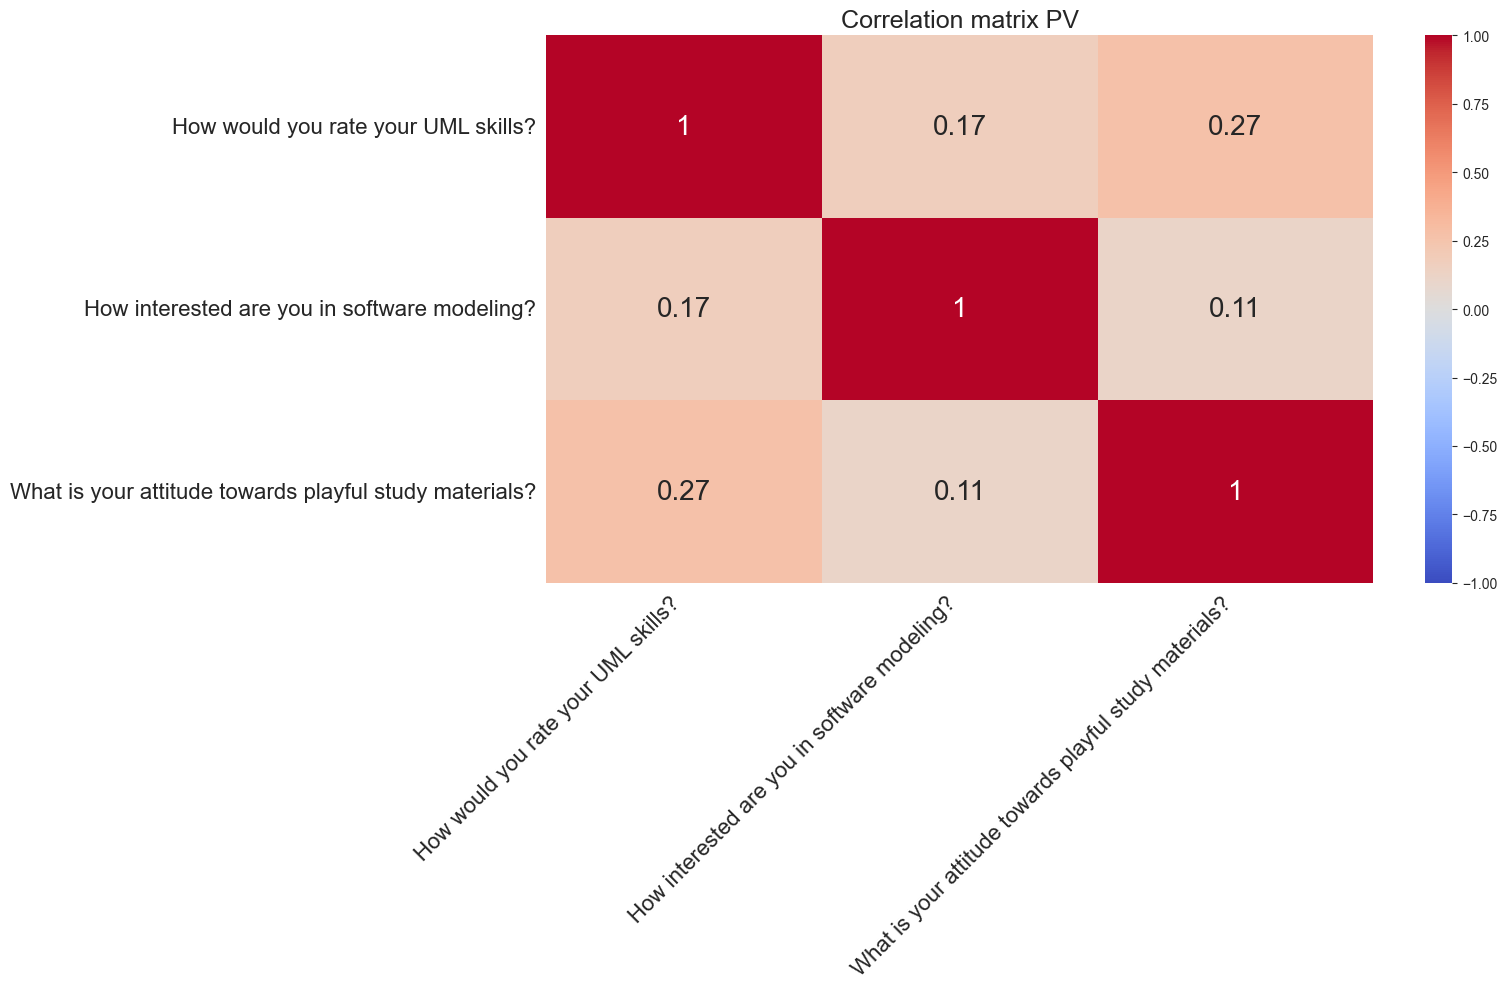
\includegraphics[width=0.85\textwidth]{assets/images/eval/engagement/corr_matrix_feedback_P_1.png}
\caption{Correlation matrix for feedback questionnaire - \ac{pv}}
\label{fig:corr_matrix_feedback_P_1}
\end{figure}
\FloatBarrier

% \textbf{Summary}

% The textual responses in \ac{pv} display a better overall reception and higher enthusiasm than \ac{cv}. This observation is further supported by the feedback questionnaire, where \ac{pv} scored higher in satisfaction and engagement across almost all numeric metrics. 

% Despite that, \ac{pv} shows a drop in interest in software modeling itself between the start and end of the course, while interest in \ac{cv} remained almost unchanged. That presents a potential trap, where flawed playful design might shift the students' motivation away from intrinsic interest, or make students take the taught topic less seriously.

% It should be noted that responses in \ac{cv} are more varying and point to a slightly polarizing effect, where some students enjoy the design very much and some find it off-putting. Responses in \ac{pv} tend to be less varying and more middle-ground, suggesting the playful design is more accessible in general.

% Competitive design might be more suitable to students who are already skilled and interested in the taught topics, while playful design is accessible to all kinds of students.

% The textual responses in \ac{pv} indicate better overall reception and higher enthusiasm than \ac{cv}, which is supported by higher satisfaction and engagement scores across most metrics.

% However, \ac{pv} shows a decrease in interest in software modeling, suggesting a potential risk of shifting motivation away from intrinsic interest if not designed carefully.

% Responses in \ac{cv} are more variable, indicating a polarizing effect, whereas \ac{pv} responses are more consistent, suggesting greater accessibility.

% Overall, competitive design appears more suitable for already skilled and interested students, while playful design is more accessible to a broader audience.